\subsection{Intercepting Applications}
The approach presented in this section relies on two building blocks: WireGuard and \ld.
WireGuard is a simple, fast and secure VPN software that transmits encrypted data encapsulated in UDP datagrams.
The use of UDP for communication eliminates the problem of TCP connection losses during handovers since neither UDP nor WireGuard is connection-oriented.
% Once an initial handover is complete, WireGuard sends the UDP datagrams over the new connection without the TCP connection tunneled through the WireGuard VPN noticing.
% To realize our approach the WireGuard software needs to be installed on the system, which can either be done as a kernel module or, if no kernel module is available (e.g., for non-Linux based systems or the kernel of the system can not be modified) as a platform-independent user space version.
% For this approach both alternative are possible.
For the WireGuard tunnel to work, an additional tunnel endpoint somewhere in the network is required, where the WireGuard tunnel is terminated and the encapsulated TCP connection further relayed to the original destination.

The use of WireGuard alone does not automatically enable existing TCP-based applications to support handovers.
Rather, they have to be instructed to transfer their data over the WireGuard connection.
One way to do this, is to modify the routing table of the system in a way, that all traffic from the host is sent over the tunnel.
However, this would mean that non-TCP based applications would also be routed through the tunnel, including UDP or QUIC based applications that do not have the problem of missing handover capability making the routing table an inappropriate interface for the TCP mechanism.
% This approach would just add the overhead of WireGuard for these applications without gaining anything.
% This is where \ld comes into play.
To mitigate this potential drawback, \ld is used.
The \ld mechanism allows intercepting functions of dynamically linked libraries, enabling to intercept the Sockets API such that only connections of the application started with our \ld modifications are using the WireGuard tunnel.
Following the model of this paper, the mechanism \emph{TCP/IP} is replaced by the mechanism \emph{TCP/Tunnel/IP}. 
For this purpose, an interceptor is created that implements the sockets API used by the system, i.e. the application.


\begin{figure}
    \centering
    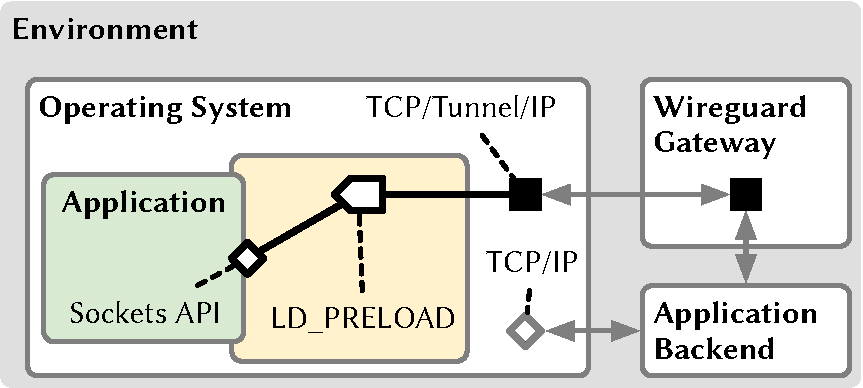
\includegraphics[width=.9\linewidth]{figures/model_TunnelHandover.pdf}
    \caption{The system architecture for the TunnelHandover approach}
    \label{fig:model_TunnelHandover}
\end{figure}
Figure\ \ref{fig:model_TunnelHandover} presentes the architectural components of the TunnelHandover approach. 
A WireGuard daemon is run on the operating system, indicated by the black square.
When a program is executed with our interceptor, the TCP packets of this particular application are intercepted and redirected to the local WireGuard daemon.
The UDP-based WireGuard packets are then sent to the WireGuard endpoint located in the network, which unpacks the encapsulated TCP connection and acts as a relay to forward the application data to the desired destination using conventional TCP/IP mechanisms.
The responses from the server with which the application is communicating are sent back to the host via the same route, i.e. via the WireGuard tunnel.
% The exact implementation and configuration will be discussed below.

% \subsection{Implementation}
% Several implementations lead to the desired result, but with different drawbacks.
% The first approach would be to configure the WireGuard in a way so that no traffic is sent through the tunnel and the \ld implementation sets a rule in the routing table that causes the traffic of an application to be sent through the WireGuard tunnel on a IP address basis.
% However, this approach has several disadvantages.
% First, three functions of the socket API must be overridden, \texttt{socket}, \texttt{connect} and \texttt{close}.
% The \texttt{socket} system call returns a file descriptor and the \texttt{connect} call connects to a given IP address over the socket with the file descriptor of the previous \texttt{socket} call.
% Once both the file descriptor and the IP address are available, the routing table has to be modified by adding a rule to route the extracted IP address over the WireGuard interface.
% This, however, has the disadvantage that other applications that have the same endpoint would also be tunneled through WireGuard.
% Finally, when the the client closes a connection, the \texttt{close} system call is used.
% the \ld implementation at this point has to remove the rule from the routing table to restore the original state.
% However, to realize this cleanup, a mapping is required between the file descriptor and the corresponding IP address leading to both implementation and runtime overhead for this mapping, as the \texttt{close} system call only closes a file descriptor.

% An alternative approach is to bind a socket to an interface using the \texttt{SO\_BINDTODEVICE} socket option.
% Using this option, the socket is advised to route all traffic that is sent to the given file descriptor using a specific interface, in our case the WireGuard interface.
% This approach has multiple advantages.
% First of all, it only requires the \texttt{socket()} system call to be overridden.
% Whenever the application opens a new TCP socket, our \ld implementation binds this socket to the WireGuard interface.
% Second, it has minimal implementation and runtime overhead, as there is no state that has to be maintained as in the above approach.
% Finally, as soon as the application closes the socket using the \texttt{close()} system call, the binding created by our \ld implementation is also removed by the Linux kernel.
% However, this approach comes with the downside that the Linux kernel has a security mechansism called \textit{Reverse Path Filtering (RPF)}.
% One of our goals is that only connections of applications using the \ld implementation are routed through the WireGuard tunnel.
% To solve this either a route for each application has to be set, which leads to the rejected solution from above.
% Alternatively, a second routing table is created for the WireGuard interface.
% If the application's socket is bound to the WireGuard interface because the application uses our \ld implementation, the Linux kernel will still send and route packets via the interface, since an entry exists for this interface in the second table.
% The problem now is that responses from the server are dropped by Linux because of said RPF.
% When the kernel receives an IP packet, it checks whether the source of the packet is reachable through the interface through which it was received.
% If the packet can be forwarded over the interface from which it came, the computer accepts the packet, otherwise it will be dropped.
% In our case the packet is not routable, because the kernel only looks in the standard routing table, but does not find an entry for the IP address.
% The solution is to use policy based routing to tell the kernel to look in the second routing table for a specific IP address range, namely that of the WireGuard interface.



One of our goals is that only connections of applications using the \ld implementation are routed through the WireGuard tunnel.
Forwarding traffic of a certain TCP socket to WireGuard is implemented using the \texttt{SO\_BINDTODEVICE} socket option.
Using this option, the socket is advised to route all traffic that is sent to the given file descriptor using a specific network interface, in our case the WireGuard network interface.
However, this approach comes with the downside that the Linux kernel has a security mechanism called \textit{Reverse Path Filtering (RPF)}, which becomes active.
To cope with this problem, a second routing table is created for the WireGuard interface.
If the application's socket is bound to the WireGuard interface, the Linux kernel will still send and route packets via the interface, since an entry exists for this interface in the second table.
In addition, policy based routing is used to tell the kernel to look in the second routing table for a specific IP address range, namely that of the WireGuard interface.
 
